% me=0 student solutions (ps file), me=1 - my solutions (sol file),
% me=2 - assignment (hw file)
\def\me{0} \def\num{1} %homework number

\def\due{September 20} %due date

\def\course{CSCI-GA.2560-001, Artificial Intelligence} 
%course name, changed only once

% **** INSERT YOUR NAME HERE ****
\def\name{Kumar Prasun}

% **** INSERT YOUR NETID HERE ****
\def\netid{kp2692}

% **** INSERT NETIDs OF YOUR COLLABORATORS HERE ****
\def\collabs{}


\iffalse

INSTRUCTIONS: replace # by the homework number.  (if this is not
ps#.tex, use the right file name)

Clip out the ********* INSERT HERE ********* bits below and insert
appropriate LaTeX code.  There is a section below for student macros.
It is not recommended to change any other parts of the code.


\fi
%

\documentclass[11pt]{article}


% ==== Packages ====
\usepackage{amsfonts}
\usepackage{latexsym}
\usepackage{fullpage}
\usepackage{amsmath}
\usepackage{enumitem}
\usepackage{graphicx}
\usepackage{subcaption}
% \setlength{\oddsidemargin}{.0in} \setlength{\evensidemargin}{.0in}
% \setlength{\textwidth}{6.5in} \setlength{\topmargin}{-0.4in}
\setlength{\footskip}{0.8in} \setlength{\textheight}{8.5in}

\newcommand{\handout}[5]{
\renewcommand{\thepage}{#1, Page \arabic{page}}
  \noindent
  \begin{center}
    \framebox{ \vbox{ \hbox to 5.78in { {\bf \course} \hfill #2 }
        \vspace{4mm} \hbox to 5.78in { {\Large \hfill #5 \hfill} }
        \vspace{2mm} \hbox to 5.78in { {\it #3 \hfill #4} }
        \ifnum\me=0
        \vspace{2mm} \hbox to 5.78in { {\it Collaborators: \collabs
            \hfill} }
        \fi
      } }
  \end{center}
  \vspace*{4mm}
}

\newcounter{pppp}
\newcommand{\prob}{\arabic{pppp}} %problem number
\newcommand{\increase}{\addtocounter{pppp}{1}} %problem number

% Arguments: Title, Number of Points
\newcommand{\newproblem}[2]{
  \ifnum\me=0
    \ifnum\prob>0 \newpage \fi
    \increase
    \setcounter{page}{1}
    \handout{\name{} (\netid), Homework \num, Problem \arabic{pppp}}
    {\today}{Name: \name{} (\netid)}{Due: \due}
    {Solutions to Problem \prob\ of Homework \num\ (#2)}
  \else
    \increase
    \section*{Problem \num-\prob~(#1) \hfill {#2}}
  \fi
}

% \newcommand{\newproblem}[2]{\increase
% \section*{Problem \num-\prob~(#1) \hfill {#2}}
% }

\def\squarebox#1{\hbox to #1{\hfill\vbox to #1{\vfill}}}
\def\qed{\hspace*{\fill}
  \vbox{\hrule\hbox{\vrule\squarebox{.667em}\vrule}\hrule}}
\newenvironment{solution}{\begin{trivlist}\item[]{\bf Solution:}}
  {\qed \end{trivlist}}
\newenvironment{solsketch}{\begin{trivlist}\item[]{\bf Solution
      Sketch:}} {\qed \end{trivlist}}
\newenvironment{code}{\begin{tabbing}
    12345\=12345\=12345\=12345\=12345\=12345\=12345\=12345\= \kill }
  {\end{tabbing}}

%\newcommand{\eqref}[1]{Equation~(\ref{eq:#1})}

\newcommand{\hint}[1]{({\bf Hint}: {#1})}
\newcommand{\note}[1]{{\bf Note to Graders}: {#1}}
% Put more macros here, as needed.
\newcommand{\room}{\medskip\ni}
\newcommand{\brak}[1]{\langle #1 \rangle}
\newcommand{\bit}[1]{\{0,1\}^{#1}}
\newcommand{\zo}{\{0,1\}}
\newcommand{\C}{{\cal C}}

\newcommand{\nin}{\not\in}
\newcommand{\set}[1]{\{#1\}}
\renewcommand{\ni}{\noindent}
\renewcommand{\gets}{\leftarrow}
\renewcommand{\to}{\rightarrow}
\newcommand{\assign}{:=}

\newcommand{\AND}{\wedge}
\newcommand{\OR}{\vee}

\newcommand{\For}{\mbox{\bf for }}
\newcommand{\To}{\mbox{\bf to }}
\newcommand{\Do}{\mbox{\bf do }}
\newcommand{\If}{\mbox{\bf if }}
\newcommand{\Then}{\mbox{\bf then }}
\newcommand{\Else}{\mbox{\bf else }}
\newcommand{\While}{\mbox{\bf while }}
\newcommand{\Repeat}{\mbox{\bf repeat }}
\newcommand{\Until}{\mbox{\bf until }}
\newcommand{\Return}{\mbox{\bf return }}
\newcommand{\Halt}{\mbox{\bf halt }}
\newcommand{\Swap}{\mbox{\bf swap }}
\newcommand{\Ex}[2]{\textrm{exchange } #1 \textrm{ with } #2}



\begin{document}

\ifnum\me=0

% Collaborators (on a per task basis):
%
% Task 1: *********** INSERT COLLABORATORS HERE *********** 
% Task 2: *********** INSERT COLLABORATORS HERE *********** 
% etc.
%

\fi

\ifnum\me=1

\handout{PS \num}{\today}{Lecturer: Paul Bethe}{Due: \due}
{Solution {\em Sketches} to Problem Set \num}

\fi

\ifnum\me=2

\handout{PS \num}{\today}{Lecturer: Paul Bethe}{Due: \due}{Problem
  Set \num}

\fi


\newproblem{BFS}{3 Points}

\noindent
Show the order of nodes visited using Breadth First Search (BFS), and the final path selected. 
Is this optimal? Why or why not?

  \ifnum\me<2
\begin{solution}      

    The order of nodes visited is:

    \begin{figure}[htbp] 
    \captionsetup[subfigure]{labelformat=empty}
        \begin{subfigure}[b]{.30\linewidth}
        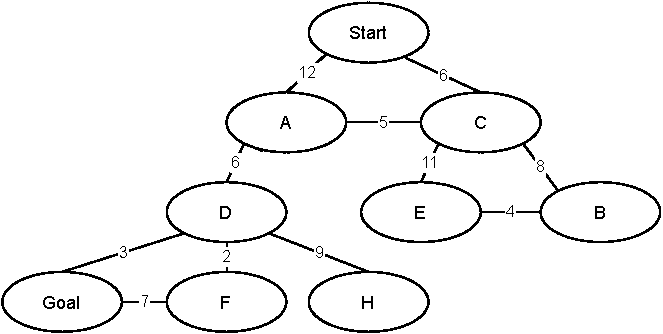
\includegraphics[width=\linewidth]{11/11_1.pdf}
        \caption{Initial Graph}\label{fig:1}
        \end{subfigure}
        \begin{subfigure}[b]{.30\linewidth}
        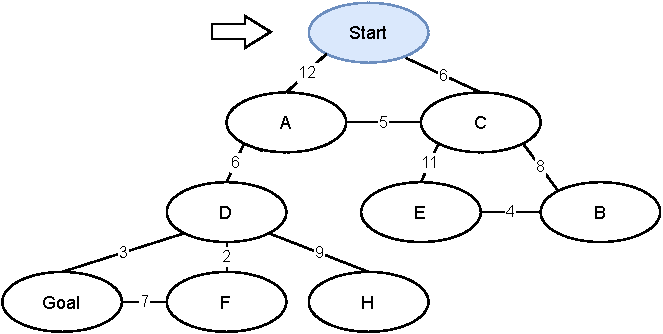
\includegraphics[width=\linewidth]{11/11_2.pdf}
        \caption{Node 1: Start}\label{fig:2}
        \end{subfigure}
        \begin{subfigure}[b]{.30\linewidth}
        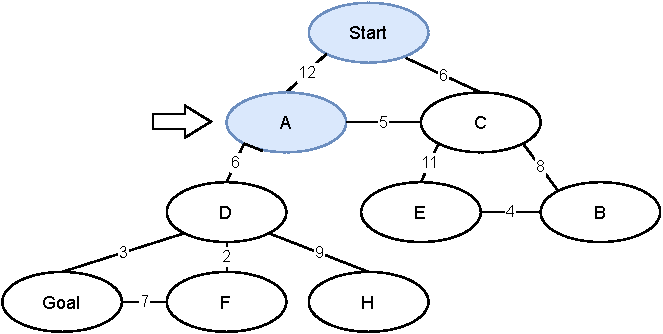
\includegraphics[width=\linewidth]{11/11_3.pdf}
        \caption{Node 2: A}\label{fig:3}
        \end{subfigure}
        \\
        \\
        \begin{subfigure}[b]{.30\linewidth}
        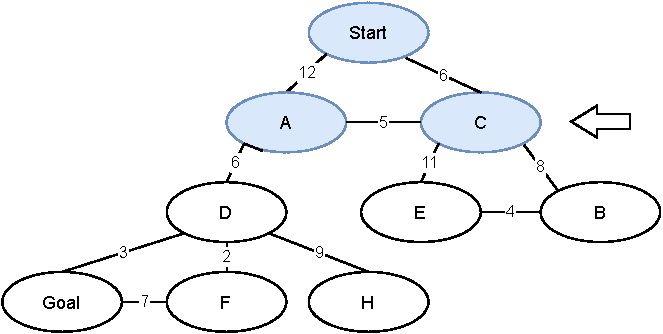
\includegraphics[width=\linewidth]{11/11_4.pdf}
        \caption{Node 3: C}\label{fig:4}
        \end{subfigure}
        \begin{subfigure}[b]{.30\linewidth}
        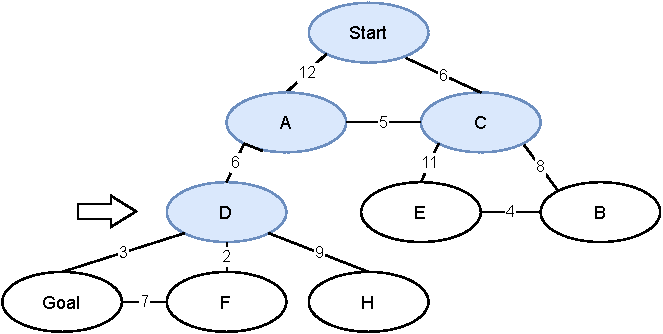
\includegraphics[width=\linewidth]{11/11_5.pdf}
        \caption{Node 4: D}\label{fig:5}
        \end{subfigure}
        \begin{subfigure}[b]{.30\linewidth}
        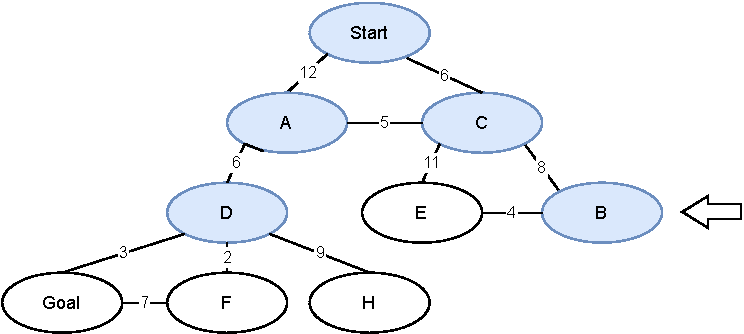
\includegraphics[width=\linewidth]{12/12_6.pdf}
        \caption{Node 5: B}\label{fig:5b}
        \end{subfigure}
        \\
        \\
        % \centering
        \begin{subfigure}[b]{.30\linewidth}
        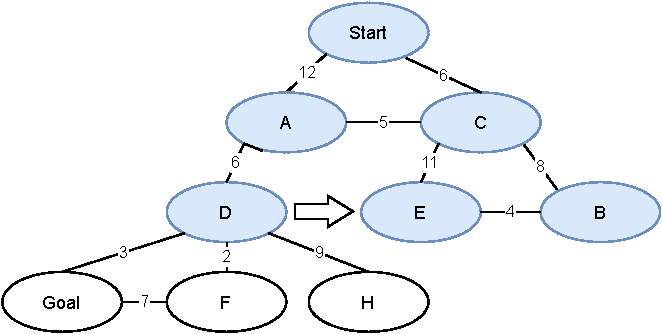
\includegraphics[width=\linewidth]{12/12_7.pdf}
        \caption{Node 6: E}\label{fig:6}
        \end{subfigure}
        \begin{subfigure}[b]{.30\linewidth}
        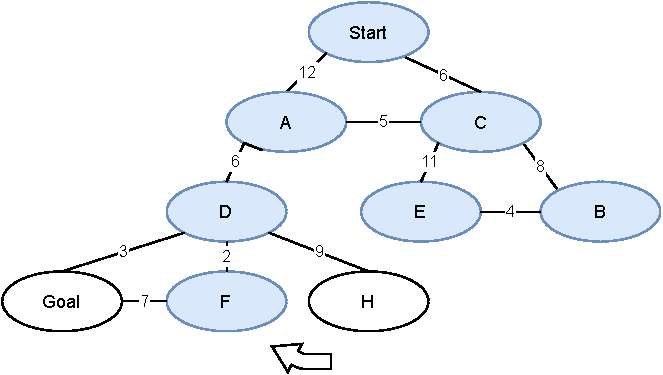
\includegraphics[width=\linewidth]{11/11_7.pdf}
        \caption{Node 7: F}\label{fig:7}
        \end{subfigure}
        \begin{subfigure}[b]{.30\linewidth}
        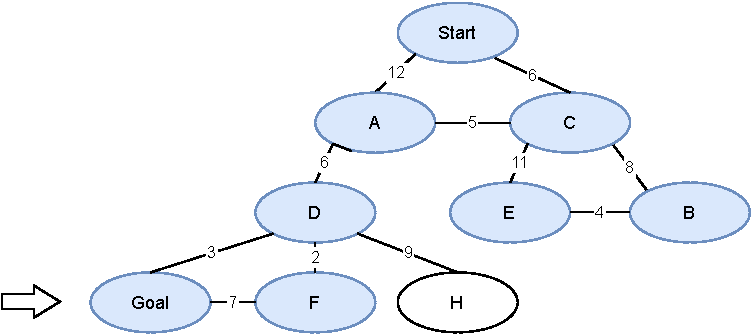
\includegraphics[width=\linewidth]{11/11_8.pdf}
        \caption{Node 8: Goal}\label{fig:8}
        \end{subfigure}
        \\
        \\
        \centering
        \begin{subfigure}[b]{.30\linewidth}
        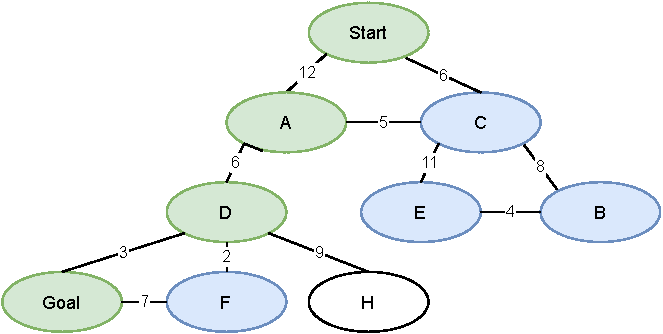
\includegraphics[width=\linewidth]{11/11_9.pdf}
        \caption{Final path selected}\label{fig:9}
        \end{subfigure}
        \caption{Order of node visits}   
        \label{fig:BFS}
    \end{figure}

    {\sc{Explanation}}:
    \begin{table}[htbp]
        \begin{tabular}{|l|l|l|l|p{0.40\linewidth}|}
        \hline
        Diagram &
          Current Path &
          Queue &
          Visited Nodes &
          Explanation \\ \hline
        Initial Graph &
          - &
          \{Start\} &
          \{\} &
          Since queue has Start, we pop and visit that node. \\ \hline
        Node 1: Start &
          Start &
          \{C,A\} &
          \{Start\} &
          A is before C in queue due to alphabetical priority. So visit node A next\\ \hline
        Node 2: A &
          Start-\textgreater{}A &
          \{D,C\} &
          \{Start,A\} &
          We visit C as it's first in queue. \\ \hline
        Node 3: C &
          Start-\textgreater{}C &
          \{E,B,D\} &
          \{Start, A, C\} &
          We visit D as it's first in queue. \\ \hline
        Node 4: D &
          Start-\textgreater{}A-\textgreater{}D &
          \begin{tabular}[c]{@{}l@{}}\{H,Goal,F,\\ E,B\}\end{tabular} &
          \begin{tabular}[c]{@{}l@{}}\{Start, A, C,\\ D\}\end{tabular} &
          We visit B as it's first in queue. \\ \hline
        Node 5: B &
          Start-\textgreater{}C-\textgreater{}B &
          \begin{tabular}[c]{@{}l@{}}\{H,Goal,F,\\ E\}\end{tabular} &
          \begin{tabular}[c]{@{}l@{}}\{Start, A, C,\\ B\}\end{tabular} &
          We visit E as it's first in queue. \\ \hline
        Node 6: E &
          Start-\textgreater{}C-\textgreater{}E &
          \{H,Goal,F\} &
          \begin{tabular}[c]{@{}l@{}}\{Start, A, C,\\ B, E\}\end{tabular} &
          We visit F as it's first in queue. \\ \hline
        Node 7: F &
          \begin{tabular}[c]{@{}l@{}}Start-\textgreater{}A-\textgreater{}D\\ -\textgreater{}F\end{tabular} &
          \{H,Goal\} &
          \begin{tabular}[c]{@{}l@{}}\{Start, A, C,\\ B, E\}\end{tabular} &
          We visit Goal as it's first in queue. \\ \hline
        Node 8: Goal &
          \begin{tabular}[c]{@{}l@{}}Start-\textgreater{}A-\textgreater{}D\\ -\textgreater{}Goal\end{tabular} &
          \{H\} &
          \begin{tabular}[c]{@{}l@{}}\{Start, A, C,\\ B, E, F\}\end{tabular} &
          We've visited Goal node. Terminate program. \\ \hline
        \end{tabular}
    \end{table}

    The green nodes highlighted in the final graph of Figure 1, are the nodes visited in the final selected path.
    The path is not optimal as it's path cost is $12+6+3=21$. The optimal path among all possible paths is
    from $Start \rightarrow C \rightarrow A  \rightarrow D \rightarrow Goal$ with a path cost of $6+5+6+3=20$.
\end{solution}
  \fi

\newproblem{Iterative Deepening}{3 Points}
\noindent
Show the order of nodes visited using Iterative Deepening (initial depth of 2, increasing depth by 1), 
and the final path selected. Is this optimal

\ifnum\me<2
\begin{solution}      

    The order of nodes visited is:
    \\ \\
    For Depth = 2
    \begin{figure}[htbp] 
    \captionsetup[subfigure]{labelformat=empty}
        \begin{subfigure}[b]{.30\linewidth}
        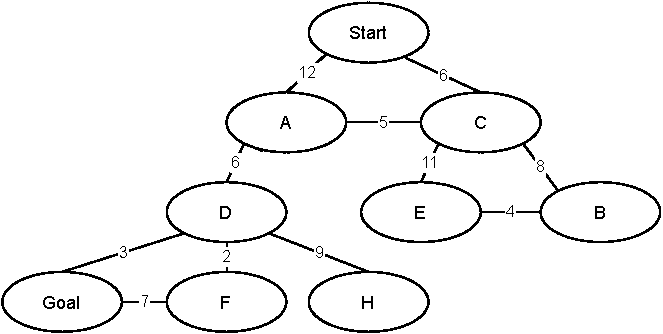
\includegraphics[width=\linewidth]{12/12_1.pdf}
        \caption{Initial Graph}\label{fig:10}
        \end{subfigure}
        \begin{subfigure}[b]{.30\linewidth}
        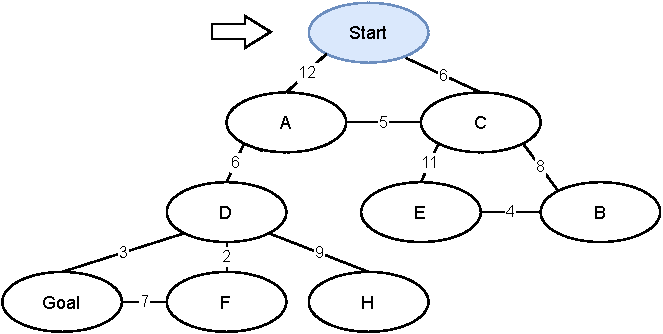
\includegraphics[width=\linewidth]{12/12_2.pdf}
        \caption{Node 1: Start}\label{fig:11}
        \end{subfigure}
        \begin{subfigure}[b]{.30\linewidth}
        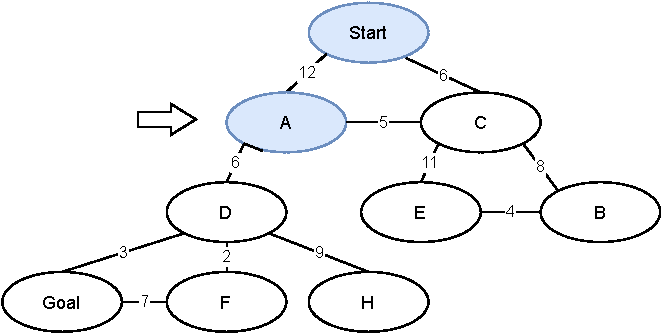
\includegraphics[width=\linewidth]{12/12_3.pdf}
        \caption{Node 2: A}\label{fig:12}
        \end{subfigure}
        \\
        \\
        \hspace*{\fill}
        {
        \begin{subfigure}[b]{.30\linewidth}
        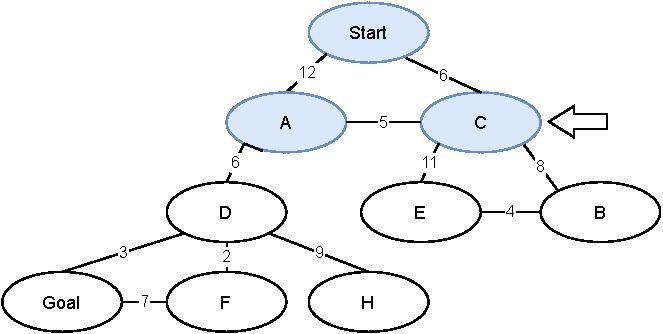
\includegraphics[width=\linewidth]{12/12_4c.pdf}
        \caption{Node 3: C}\label{fig:13}
        \end{subfigure}
        \hfill
        \begin{subfigure}[b]{.30\linewidth}
        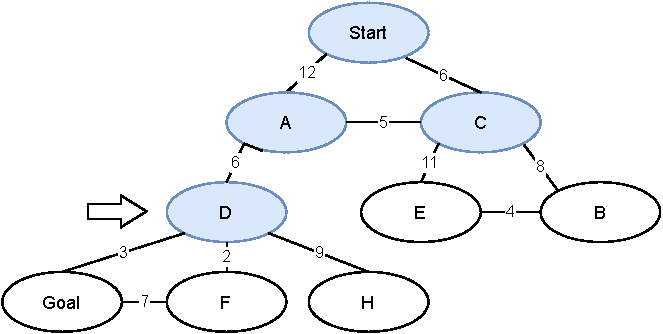
\includegraphics[width=\linewidth]{12/12_5d.pdf}
        \caption{Node 4: D}\label{fig:14}
        \end{subfigure}
        }
        \hspace*{\fill}

        \caption{Order of node visits for depth = 2}   
        \label{fig:IDS}
    \end{figure}

    {\sc{Explanation}}:
    The IDS algorithm tries to go to the deepest level of the tree till it reaches the goal 
    or depth limit. The order in which the children nodes are traversed is based on alphabetical priority.
     
    Nodes E and B will be not be visited since they are can only be reached from path 
    $ Start-\textgreater{}A-\textgreater{}C $, but the depth limit (of 2) has been reached.

    They cannot be reached from path $ Start-\textgreater{}C $ as Node C has already been visited via path
    $ Start-\textgreater{}A-\textgreater{}C $  and so the former path will be ignored by IDS due to Node C already 
    being in the visited set.
    
    \newpage
    For Depth = 3
    \begin{figure}[htbp] 
    \captionsetup[subfigure]{labelformat=empty}
        \begin{subfigure}[b]{.30\linewidth}
        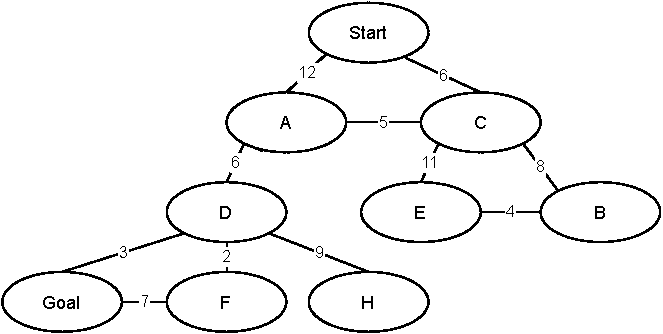
\includegraphics[width=\linewidth]{12/12_1.pdf}
        \caption{Initial Graph}\label{fig:17}
        \end{subfigure}
        \begin{subfigure}[b]{.30\linewidth}
        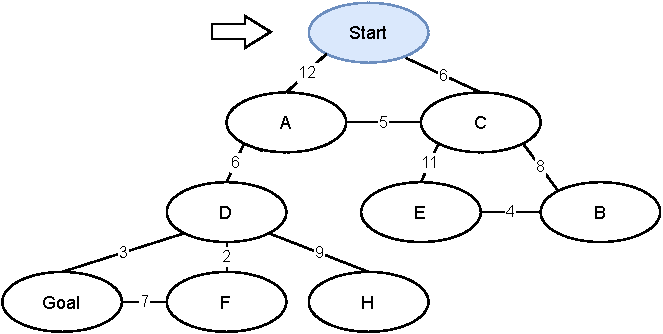
\includegraphics[width=\linewidth]{12/12_2.pdf}
        \caption{Node 1: Start}\label{fig:18}
        \end{subfigure}
        \begin{subfigure}[b]{.30\linewidth}
        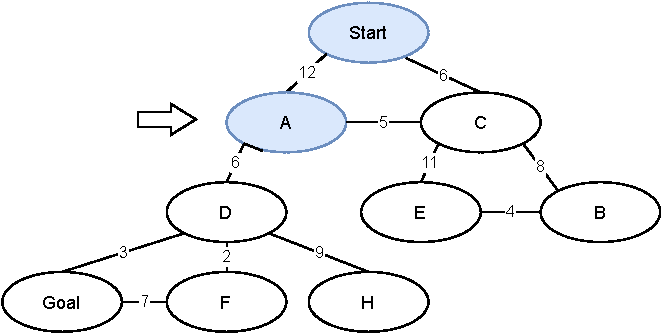
\includegraphics[width=\linewidth]{12/12_3.pdf}
        \caption{Node 2: A}\label{fig:19}
        \end{subfigure}
        \\
        \\
        \begin{subfigure}[b]{.30\linewidth}
        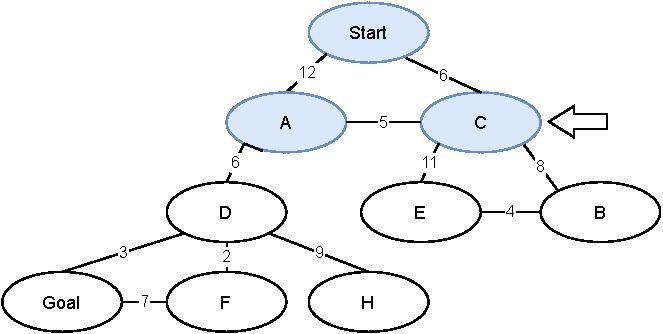
\includegraphics[width=\linewidth]{12/12_4c.pdf}
        \caption{Node 3: C}\label{fig:20}
        \end{subfigure}
        \begin{subfigure}[b]{.30\linewidth}
        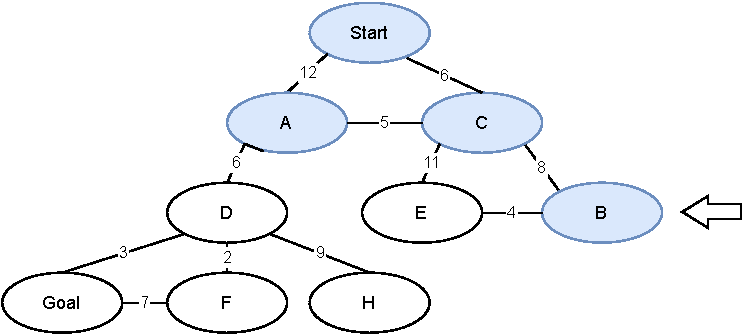
\includegraphics[width=\linewidth]{12/12_5c.pdf}
        \caption{Node 4: B}\label{fig:21}
        \end{subfigure}
        \begin{subfigure}[b]{.30\linewidth}
            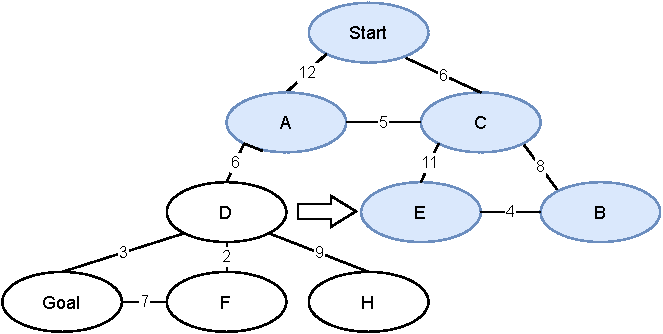
\includegraphics[width=\linewidth]{12/12_6c.pdf}
            \caption{Node 5: E}\label{fig:22}
        \end{subfigure}

        \begin{subfigure}[b]{.30\linewidth}
        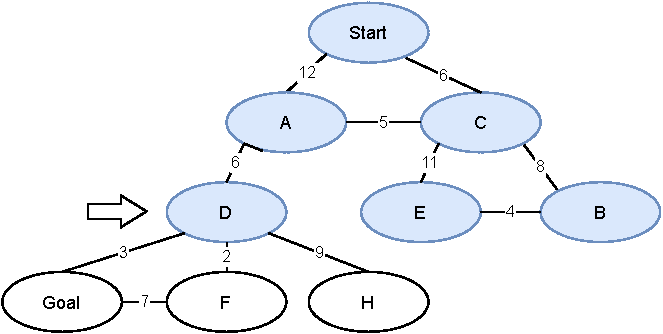
\includegraphics[width=\linewidth]{12/12_7c.pdf}
        \caption{Node 6: C}\label{fig:23}
        \end{subfigure}
        \begin{subfigure}[b]{.30\linewidth}
        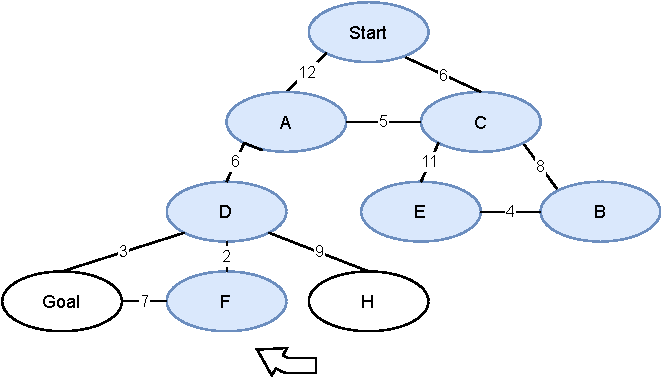
\includegraphics[width=\linewidth]{12/12_8c.pdf}
        \caption{Node 7: F}\label{fig:24}
        \end{subfigure}
        \begin{subfigure}[b]{.30\linewidth}
            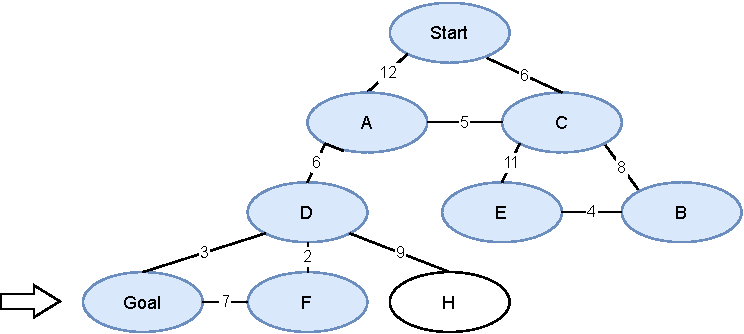
\includegraphics[width=\linewidth]{12/12_9c.pdf}
            \caption{Node 8: Goal}\label{fig:25}
        \end{subfigure}
        \\
        \\
        \centering
        \begin{subfigure}[b]{.30\linewidth}
        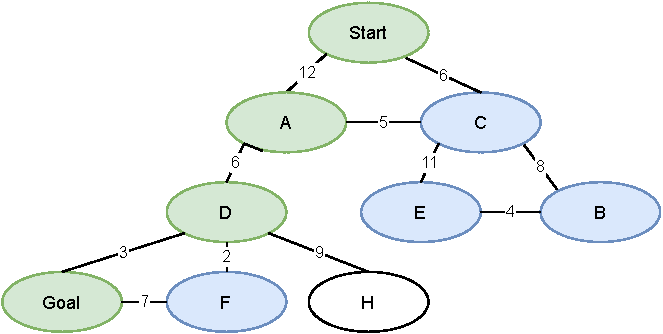
\includegraphics[width=\linewidth]{11/11_9.pdf}
        \caption{Final path selected}\label{fig:26}
        \end{subfigure}

        \caption{Order of node visits for depth = 3}   
        \label{fig:IDS_2}
    \end{figure}
    \\
        The green nodes highlighted in the final graph of Figure 3, are the nodes visited in the final selected path.
        The path is not optimal as it's path cost is $12+6+3=21$. The optimal path among all possible paths is
        from $Start \rightarrow C \rightarrow A  \rightarrow D \rightarrow Goal$ with a path cost of $6+5+6+3=20$.
\end{solution}
  \fi
\newproblem{A*}{4 Points}
\noindent
Using the above h-function, show the order of nodes visited using A*,and the final 
path selected. Is this optimal? Why or why not?

\ifnum\me<2
\begin{solution}      

    The order of nodes visited is:
    \\ \\
    \begin{figure}[htbp] 
    \captionsetup[subfigure]{labelformat=empty}
        \begin{subfigure}[b]{.30\linewidth}
        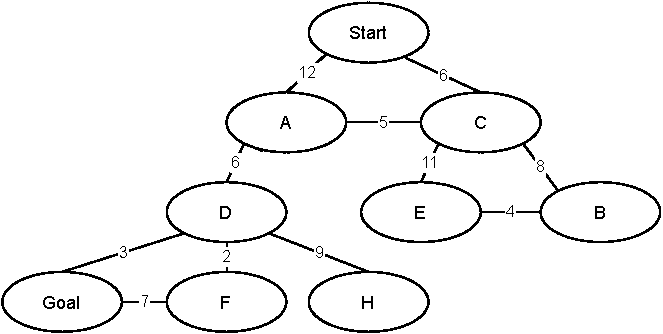
\includegraphics[width=\linewidth]{11/11_1.pdf}
        \caption{Initial Graph}\label{fig:27}
        \end{subfigure}
        \begin{subfigure}[b]{.30\linewidth}
        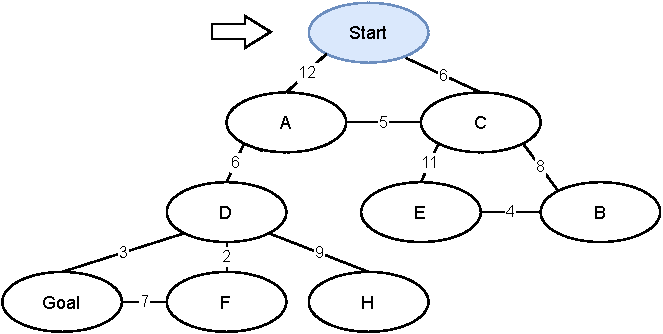
\includegraphics[width=\linewidth]{11/11_2.pdf}
        \caption{Node 1: Start}\label{fig:28}
        \end{subfigure}
        \begin{subfigure}[b]{.30\linewidth}
        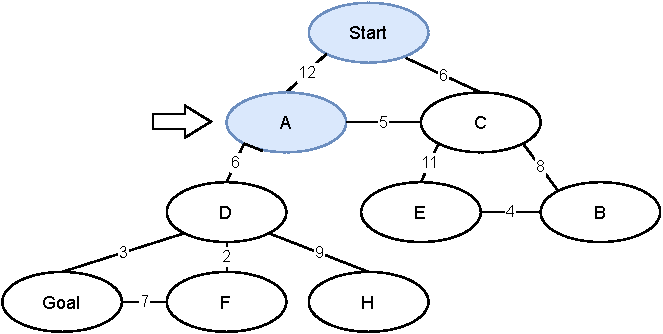
\includegraphics[width=\linewidth]{11/11_3.pdf}
        \caption{Node 2: A}\label{fig:29}
        \end{subfigure}
        \\
        \\
        \begin{subfigure}[b]{.30\linewidth}
        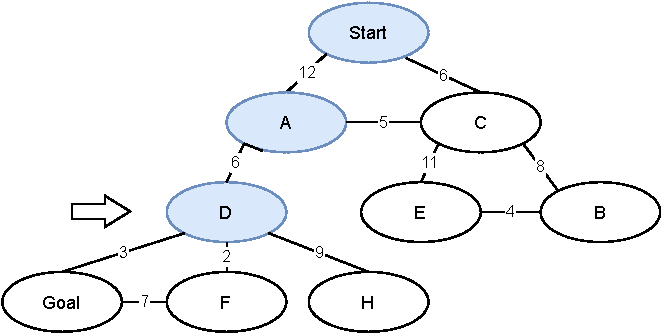
\includegraphics[width=\linewidth]{12/12_4.pdf}
        \caption{Node 3: D}\label{fig:30}
        \end{subfigure}
        \begin{subfigure}[b]{.30\linewidth}
        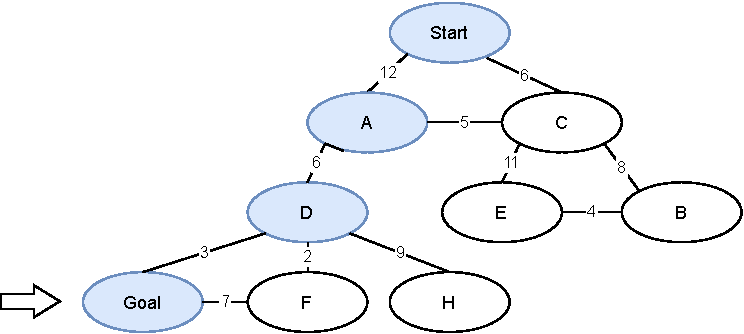
\includegraphics[width=\linewidth]{13/13_5.pdf}
        \caption{Node 4: Goal}\label{fig:31}
        \end{subfigure}
        \begin{subfigure}[b]{.30\linewidth}
        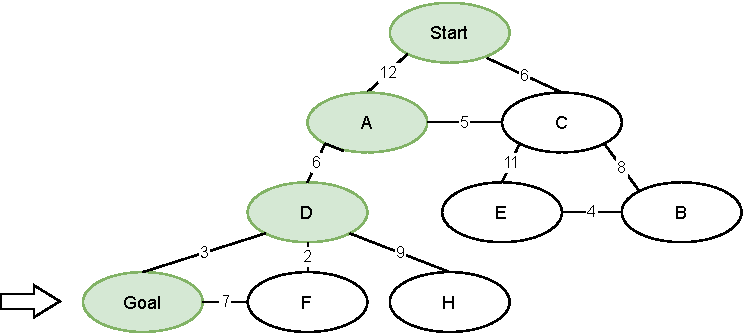
\includegraphics[width=\linewidth]{13/13_6.pdf}
        \caption{Final path selected}\label{fig:32}
        \end{subfigure}

        \caption{Order of node visits for A*}   
        \label{fig:A*}
    \end{figure}
    \\
    \begin{table}[htbp]
    \resizebox{\textwidth}{!}{%
    \begin{tabular}{|l|l|l|}
    \hline
    Diagram  & f(n) Value   & Explanation                                                      \\ \hline
    Node 2:A & = 12 + 9 =21 & This is less than that of Node C, f(Start-\textgreater{}C) = 22. \\ \hline
    Node 3:D    & = 18 + 2 =20 & This is less than that of Node C, f(Start-\textgreater{}C) = 22 \& f(Start-\textgreater{}A-\textgreater{}C) = 33. \\ \hline
    Node 4:Goal & = 21 + 0 =21 & This is less than f(n) of all other nodes in the priority queue. Program terminates.                              \\ \hline
    \end{tabular}%
    }
    \end{table}
    \\
        The green nodes highlighted in the final graph of Figure 4, are the nodes visited in the final selected path.
        The path is not optimal as it's path cost is $12+6+3=21$. The optimal path among all possible paths is
        from $Start \rightarrow C \rightarrow A  \rightarrow D \rightarrow Goal$ with a path cost of $6+5+6+3=20$.
\end{solution}
  \fi


\end{document}
